\documentclass[12pt]{notes}

% Command for Questions
%\question{}

% Command for Notes
% \note{}

% Code to create a minipage where you can type in class notes. 
%%\begin{minipage}[l][2cm][c]{\textwidth}
%\begin{comment}

%\end{comment}
%%\end{minipage}


% Begin Document
%==============================================================================
\begin{document}
% Include the Title of the Handout
\ntitle{3.2: Variable Selection}

\section{Why Variable Selection}
\bi
\item Up until now, we have focused on trying to make predictions/inference using all the potential explanatory variables we have available to us. 
\item We now wish to consider several candidate models, ultimately making a judgment as to which model is ``best.''
\bi
\item Selection is more than an art than it is a science: no ``right'' decisions, several \textit{wrong} decisions, several ``reasonables.''
\item This is an iterative process, that makes it difficult to know when we are ``done'' (see Figure \ref{fig:workflow} on last page). 
\ei
\item One element of the model building process involves \textbf{selecting a subset} of potential explanatory variables for use in the final model. 
\bi
\item Follows the Ockham's razor principle:  \emph{entia non sunt multiplicanda praeter necessitatem}
\ei
\begin{minipage}[l][2cm][c]{\textwidth}
%\begin{comment}
\note{``Entities should not be multiplied without necessity'' (i.e. all else equal: simpler answers are better).}
%\end{comment}
\end{minipage}
\ei



\question{(Groups) Why might we prefer simpler models to complex ones? \textit{Should} we prefer simpler models to more complex ones?}

\begin{minipage}[l][4cm][c]{\textwidth}
%\begin{comment}
\note{
\bi
\item Simpler models are easier to interpret/describe. 
\item Simpler models are harder to overfit. 
\item \textit{Conversely,} simpler models may fail to describe a complex problem. 
\ei
}
%\end{comment}
\end{minipage}

\question{(Groups) Why is variable selection not something we would normally want to use in an experimental setting?}

\begin{minipage}[l][3cm][c]{\textwidth}
%\begin{comment}
\note{Observational studies are usually searching to find \textit{something} interesting, while in an experiment, we wish to test whether \textit{specific things} are interesting. In experiments, we should have decided beforehand what factors we were going to control for.}
%\end{comment}
\end{minipage}

\section{Methods of Variable Selection}
How to pick the ``best'' subset of variables? 
\bi
\item Whenever possible, remove variables based on \textbf{context}, which comes with \textbf{expertise}.
\item Automatic Methods:
\bi
\item \textbf{All possible regressions:} Consider all possible combinations of predictor variables, select the ``best'' model according to some measurement criteria.  
\item \textbf{Stepwise methods:} Take a structured approach that takes a (semi) intelligent search through a subset of all possible models. 
\item \textbf{Penalized regression:} more in Module 4. 
\ei 
\ei

\subsection{All Possible Regressions}
Consider all subsets of predictor variables $X_1,  \ldots , X_{p-1}$. 

\bi
\item Number of subsets of size $p-1 = \binom{P-1}{p-1} = \frac{(P-1)!}{(p-1)!(P-p)!}$.
\item Number of subsets of all possible sizes: $\sum_{p=1}^P \binom{P-1}{p-1} = 2^{P-1}$.
\ei

\subsubsection{Measures of ``goodness''}
\begin{itemize}
     \item R-square - but which model will always have the highest $R^2$?
        \begin{eqnarray}
           R^2_p & = & 1 - \frac{SS_{Error,p}}{SS_{Total}} \nonumber
        \end{eqnarray}
     \item Adjusted R-square - balances against \# of predictors
        \begin{eqnarray}
           R^2_{a,p} & = & 1 - \frac{n-1}{n-p}\cdot\frac{SS_{Error,p}}{SS_{Total}} \nonumber
        \end{eqnarray}
       As $p$ increases, $R^2_{a,p}$ first increases, then decreases
     \item Mallow's $C_p$ - for a certain subset of $p-1$ predictors:
        \begin{eqnarray}
           C_p & = & \frac{\mbox{$SS_{Error}$ from model with $p-1$ predictors}}{\mbox{$MSE$ from model with $P-1$ predictors}} + 2p - n \nonumber
        \end{eqnarray}
        When a subset of $p-1$ predictors gives unbiased $\hat{Y}$'s, $E[C_p] \approx p$.\\
     -- so look for model with smallest $p$ such that $C_p \approx p$,\\ i.e., want $C_p \approx$ \# predictors + 1.
    \item Akaike's information criteria \& Schwarz's Bayesian criterion\\
    -- both penalize larger numbers of predictors (want small):
        \begin{eqnarray}
           AIC_p & = & n \log SS_{Error,p} - n \log n + 2 p \nonumber \\
           SBC_p & = & n \log SS_{Error,p} - n \log n + p \log n \nonumber
        \end{eqnarray}
    \item Prediction sum of squares -- based on leave-one-out philosophy ($\hat{Y}_{i(i)}$)
       \begin{eqnarray}
          PRESS_p & = & \sum_{i=1}^n \left(Y_i - \hat{Y}_{i(i)} \right)^2 \nonumber
       \end{eqnarray}
    -- look for models with small $PRESS_p$
    \end{itemize}

\subsection{Stepwise Selection}

Stepwise methods:
 \begin{itemize}
   \item automatically select a model based on some criterion
   (convenient)
   \item less satisfactory, do not ``guarantee'' the ``right'' model
   \item best used as ``confirmatory'' approaches
   \item three main: backward (okay), forward (worst), stepwise (hybrid)
 \end{itemize}

\vspace{1em}

Backward Elimination -- basic algorithm
\begin{enumerate}
   \item Fit model with all $P-1$ predictors
     \begin{enumerate}
        \item Compare each predictor's individual P-value to some
   threshold (\verb7slstay7; default in SAS is 0.10)
        \item If any predictor's P-value $>$ \verb7slstay7, drop
   predictor with largest P-value
      \end{enumerate}
   \item Repeat with $P-2$ predictors
   \item Continue until all predictors remaining have P-values below
   \verb7slstay7
\end{enumerate}

\vspace{1em}

Forward Selection -- basic algorithm
\begin{enumerate}
  \item Find predictor with highest correlation with response
    \begin{enumerate}
      \item Regress response on this predictor
      \item Leave predictor in model if
      P-value is below some threshold (\verb7slentry7; default in
      SAS is 0.50)
    \end{enumerate}
  \item Given the previously entered predictor, find the predictor
  with the highest partial correlation with response
    \begin{enumerate}
      \item Add this predictor to the model
      \item Leave in model if P-value is below \verb7slentry7
    \end{enumerate}
  \item Continue until no more predictors warrant inclusion\\
   (P-value of ``next'' predictor above threshold)
\end{enumerate}
Big problem here: best 2-variable model does not necessarily contain best 1-variable model
   (first step(s) can throw everything off)


Stepwise Selection -- basic  algorithm:
\begin{enumerate}
  \item Take a ``forward'' step: add ``best'' predictor with P-value below \verb7slentry7 (default 0.15)
  \item Take a ``backward'' step: evaluate all predictors in model and drop the variable with the highest P-value above \verb7slstay7 (default 0.15)
  \item Iterate ``forward'' and ``backward'' steps until model stays the same
\end{enumerate}

\vspace{1em}

Note: in all these automatic stepwise procedures (backward, forward,
stepwise), the \verb7slentry7 and \verb7slstay7 thresholds are
deceptive. After the first step (really a hypothesis test), they are
\underline{not} significance levels ($\alpha$), but ``conditional''
significance levels, which are harder to interpret.

\question{(Individual) Clearly, it would be better to compare all possible models, rather than a subset (in stepwise methods). Why do stepwise methods even exist?}


\begin{minipage}[l][2cm][c]{\textwidth}
%\begin{comment}
\note{When $P$ gets large, fitting $2^{P-1}$ models quickly becomes unrealistic computationally. Also, chance of a ``consensus'' among measurement techniques as to which is the best model becomes unlikely.}
%\end{comment}
\end{minipage}


\subsection{Remember this...}
\bi
\item In order to have reliable results, we need $n >> P$ (often 6*10 times larger). 
\item Each described technique measures how well your models fit the data you already have, which might not translate to new data (in production). 
\ei

We get a sense of how our models perform on new data by:
\bi
\item Splitting our data into ``training'' and ``test'' sets. 
\item Fit each model using only the training data, then use the model to predict on the test data. 
\item Calculate the mean square prediction error:
\begin{equation*}
      MSPR  =  \frac{\sum_{i=1}^{n^*} \left(Y_i - \hat{Y}_i  \right)^2}{n^*} \nonumber
\end{equation*}
\ei








\begin{figure}
\centering
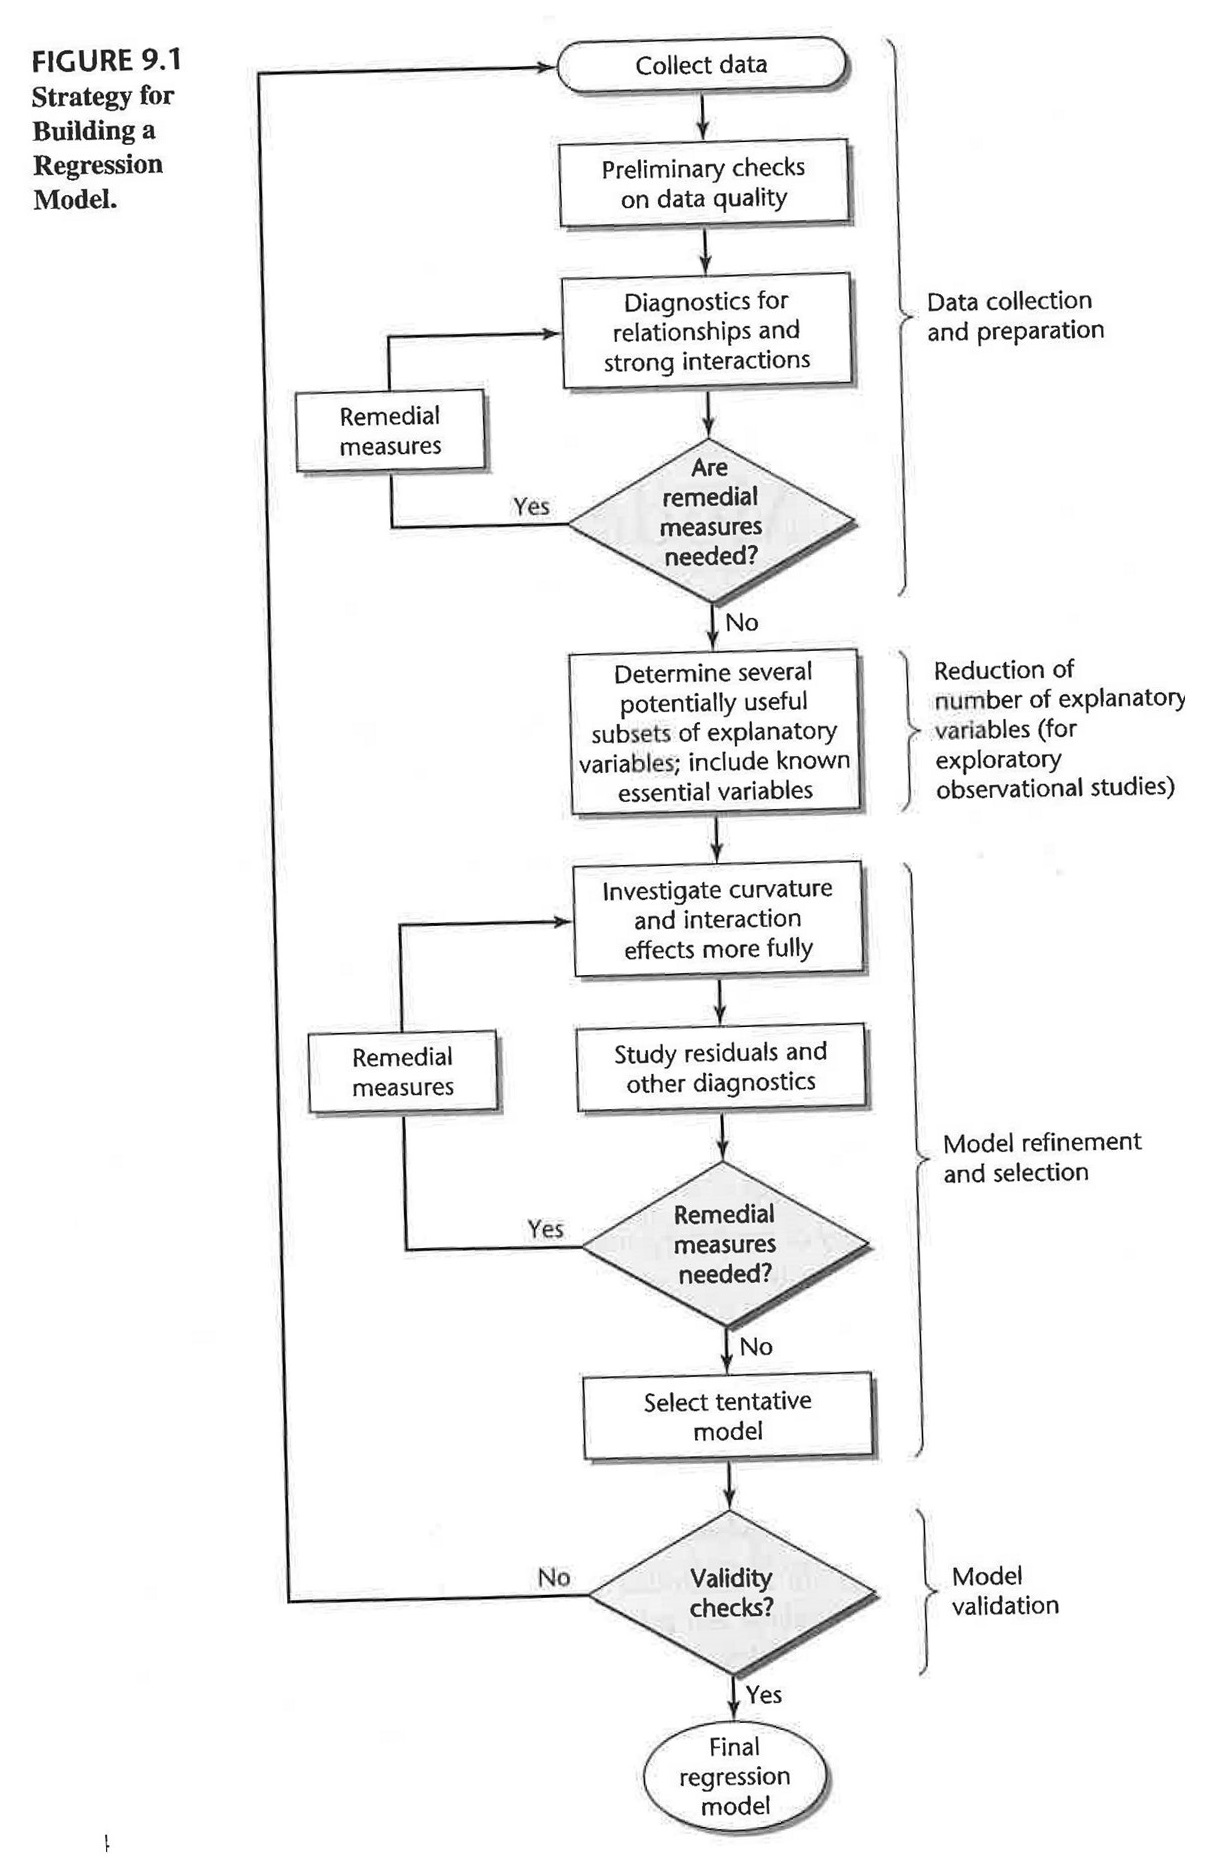
\includegraphics[width=0.9\textwidth]{figures/module3/workflow.jpg}
\caption{General model for multiple regression model selection (taken from Kutner et. al. (2004)).}
\label{fig:workflow}
\end{figure}

% End the Document
%==============================================================================
\end{document}